\section{Darstellung einer Bewegungssequenz}

Die geforderte PTP Bewegung des Roboters soll die Zeitstempel 1:05 bis 1:08 im Beispielvideo umfassen.
Die daraus resultierende Start- und Endposition ist in den Abbildungen \ref{fig:start_pos} und \ref{fig:end_pos} zusehen.
Die Startposition ist mittig an der Türe, die Endposition an der Steuerung auf der rechten Seite. 
Nach Erreichen der Endposition betätigt der Roboter einen Taster mit seinem am Greifer montierten Zylinderstift und startet dadurch die Werkstückbearbeitung in der Maschine.
Diese Tasterbetätigung ist in der Bewegungssequenz ebenfalls umgesetzt.

\begin{figure}
	\centering
	\begin{subfigure}[b]{0.496\textwidth}
		\centering
		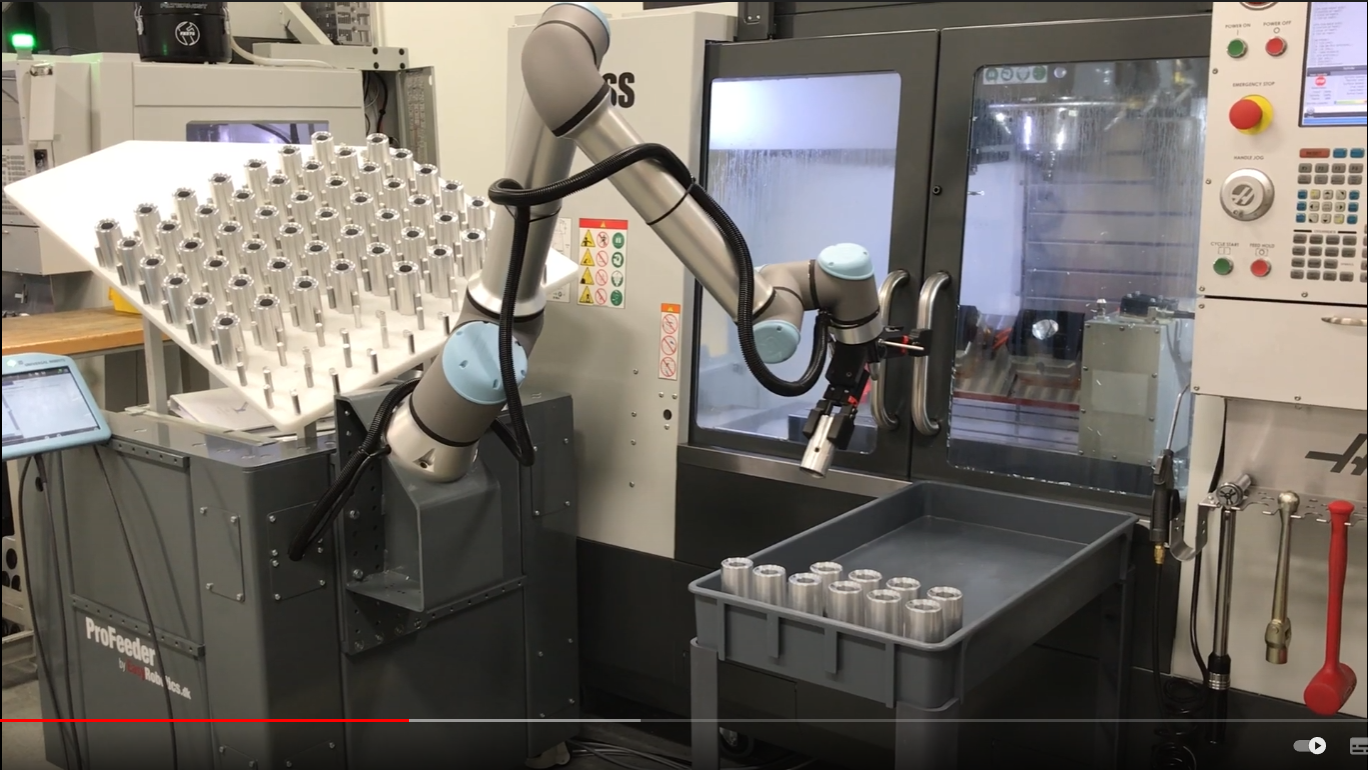
\includegraphics[width=1.0\linewidth]{grafic/ptp_startposition}
		\caption{Startposition}
		\label{fig:start_pos}
	\end{subfigure}
	\begin{subfigure}[b]{0.496\textwidth}
		\centering
		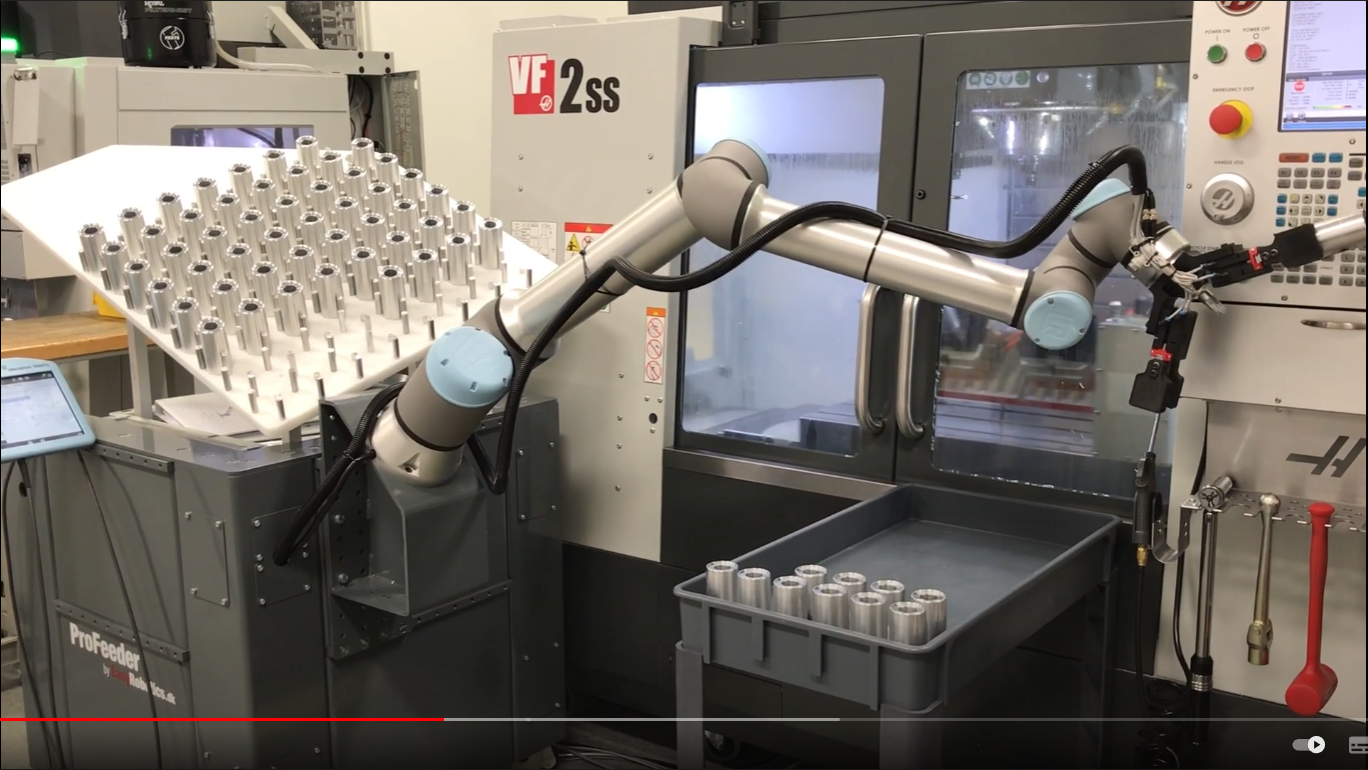
\includegraphics[width=1.0\linewidth]{grafic/ptp_endposition}
		\caption{Endposition}
		\label{fig:end_pos}
	\end{subfigure}
\caption{Start- und Endposition der PTP Bewegung, \\ Quelle: \url{https://www.youtube.com/watch?v=ugxDTtmykE4}}
\label{fig:start_end_pos}
\end{figure}


Die Bewegung ist mittels separater Ansteuerung jeder Gelenkachse realisiert.
Dazu wird ein Block namens \en{Polynominal Trajectory} verwendet, welcher Trajektorien durch gegebene Weg- und Zeitpunkte generiert.
Der verwendete Block ist in Abbildung \ref{fig:ur10_trajectoriengenerator} auf der linken Seite zu sehen.
In unserem Fall handelt es sich bei den Wegpunkten um Winkelstellungen des Gelenks.
Daher ist nach dem Trajektoriengenerator ein \en{Simulink-PS-Converter} eingefügt, der das resultierende einheitenlose Signal des Generators in ein pysikalisches mit der Einheit Rad umwandelt.

\begin{figure}[!htbp]
	\centering
	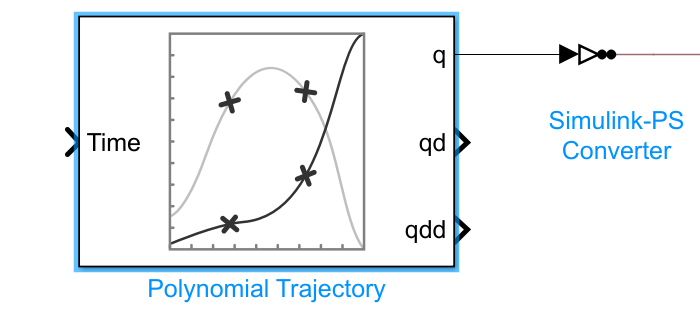
\includegraphics[width=0.55\linewidth]{grafic/Trajectoriengenerator}
	\caption{Blockdiagramm des Aktuators des ersten Gelenks}
	\label{fig:ur10_trajectoriengenerator}
\end{figure}





\newpage
\begin{figure}[!htbp]
	\centering
	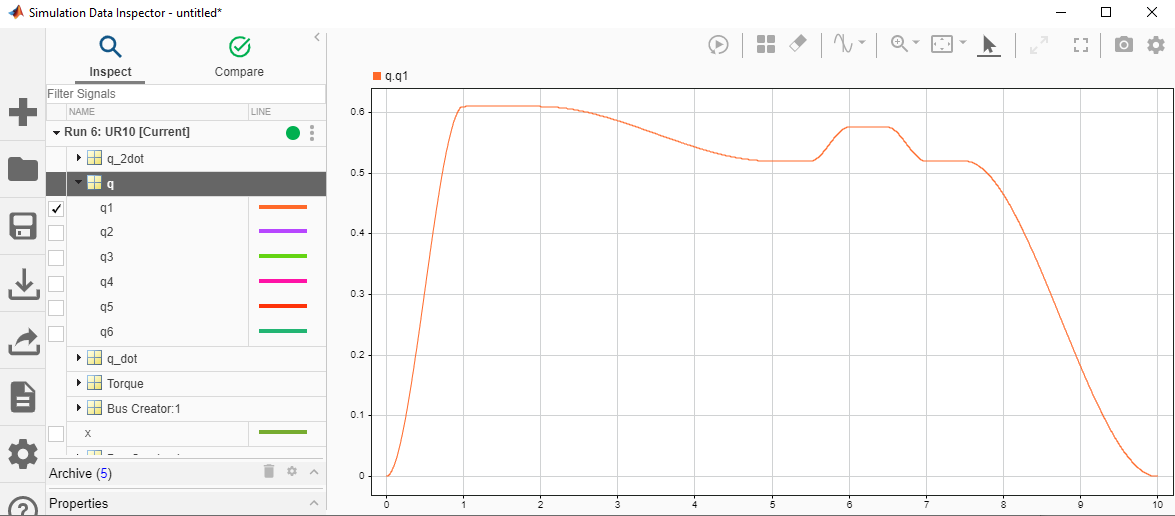
\includegraphics[width=1.0\linewidth]{grafic/data_inspector_Winkel_erstes_Gelenk}
	\caption{Winkelverlauf über Zeit des ersten Gelenks}
	\label{fig:data_inspector_rotation_angle}
\end{figure}

